% ============================================================
% Psych-Bench Supplementary Material
% Complete benchmark inventory (Table S1)
% ============================================================
\documentclass[10pt,landscape]{article}

\usepackage[margin=0.75in]{geometry}
\usepackage{longtable}
\usepackage{booktabs}
\usepackage{array}
\usepackage{hyperref}
\usepackage[T1]{fontenc}
\usepackage[utf8]{inputenc}
\usepackage{microtype}
\usepackage{amsmath}
\usepackage{pgfplots}
\usepackage{pgfplotstable}
\pgfplotsset{compat=1.18}
\usepackage[authoryear,round]{natbib}

\newcommand{\psychbench}{\textsc{Psych-Bench}}
\newcommand{\hlb}{\textsc{HLB}}

\title{\psychbench{}: Supplementary Material\\
\large Complete Benchmark Inventory}

\author{Tristan Stoltz\\
Luminous Dynamics\\
\texttt{tristan.stoltz@evolvingresonantcocreationism.com}}

\date{}

\begin{document}
\maketitle

\section*{Table S1: Complete Benchmark Inventory}

Table~S1 lists all 141 benchmarks in the \psychbench{} suite, organized by domain. Each entry provides the benchmark name, source paradigm, primary citation, year, key metric, and HDC stimulus adapter type used for encoding.

\renewcommand{\arraystretch}{1.15}
\begin{longtable}{@{}p{2.3cm}p{3.0cm}p{4.5cm}p{0.6cm}p{3.8cm}p{1.8cm}@{}}
\caption{Complete inventory of all 141 benchmarks in \psychbench{}, organized by domain.} \label{tab:s1} \\
\toprule
\textbf{Domain} & \textbf{Benchmark} & \textbf{Paradigm / Citation} & \textbf{Year} & \textbf{Key Metric} & \textbf{HDC Adapter} \\
\midrule
\endfirsthead
\toprule
\textbf{Domain} & \textbf{Benchmark} & \textbf{Paradigm / Citation} & \textbf{Year} & \textbf{Key Metric} & \textbf{HDC Adapter} \\
\midrule
\endhead
\midrule
\multicolumn{6}{r}{\emph{Continued on next page}} \\
\endfoot
\bottomrule
\endlastfoot

% --- Executive (7) ---
Executive & Stroop & Color-word interference \citep{stroop1935interference} & 1935 & stroop\_effect & Sequence \\
Executive & WCST & Set-shifting \citep{berg1948simple} & 1948 & categories\_completed & Sequence \\
Executive & Flanker & Response conflict \citep{eriksen1974effects} & 1974 & flanker\_effect & Sequence \\
Executive & Iowa Gambling & Decision under ambiguity \citep{bechara1994insensitivity} & 1994 & overall\_net\_score & Reward \\
Executive & Ravens & Fluid intelligence \citep{raven1938progressive} & 1938 & overall\_accuracy & Spatial \\
Executive & Tower of London & Planning \citep{shallice1982specific} & 1982 & overall\_optimal\_rate & Spatial \\
Executive & Dual-Task & Divided attention \citep{pashler1994dual} & 1994 & dual\_task\_cost & Sequence \\

\midrule
% --- Working Memory (6) ---
WorM & N-back & Working memory updating \citep{jaeggi2010relationship} & 1958 & nback\_2::accuracy & Sequence \\
WorM & Change Detection & Visual WM capacity \citep{luck1997capacity} & 1997 & change\_detection\_k4 & Spatial \\
WorM & Serial Recall & Short-term memory \citep{murdock1962serial} & 1962 & primacy\_advantage & Sequence \\
WorM & Spatial Updating & Spatial WM \citep{oberauer2003selective} & 2003 & updating\_accuracy & Spatial \\
WorM & Binding & Feature binding \citep{luck1997capacity} & 1997 & binding\_accuracy & Spatial \\
WorM & Digit Span & Verbal WM \citep{wechsler2008wais} & 1997 & forward\_span & Sequence \\

\midrule
% --- Memory Agent (5) ---
MemoryAgent & Accurate Retrieval & Retrieval accuracy (Anderson, 1983) & 1983 & retrieval\_accuracy & Scenario \\
MemoryAgent & Test-Time Learning & Test-enhanced learning & 2006 & online\_gain & Scenario \\
MemoryAgent & Long-Range & Long-range retention & 1885 & retention\_accuracy & Scenario \\
MemoryAgent & Conflict Resolution & Interference resolution & 1996 & resolution\_accuracy & Scenario \\
MemoryAgent & Prospective Memory & Future intention execution & 1990 & pm\_hit\_rate & Scenario \\

\midrule
% --- Attention (3) ---
Attention & Visual Search & Feature/conjunction search & 1980 & feature\_search\_accuracy & Spatial \\
Attention & Attentional Blink & Dual-target RSVP & 1992 & t1\_accuracy & Sequence \\
Attention & Mismatch Negativity & Deviance detection & 1978 & mismatch\_amplitude & Sequence \\

\midrule
% --- Sustained Attention (3) ---
SustAttn & SART & Sustained attention \citep{robertson1997sustained} & 1997 & sart\_d\_prime & Sequence \\
SustAttn & PVT & Vigilance & 1985 & pvt\_mean\_rt & Sequence \\
SustAttn & CPT & Continuous performance & 1956 & cpt\_hit\_rate & Sequence \\

\midrule
% --- Social (6) ---
Social & RME & Emotion recognition \citep{baroncohen2001eyes} & 2001 & rme\_accuracy & Scenario \\
Social & Ultimatum Game & Social fairness \citep{guth1982experimental} & 1982 & offer\_ratio & Reward \\
Social & Social Norm & Norm compliance & 2006 & norm\_detection\_accuracy & Scenario \\
Social & Prisoner's Dilemma & Cooperation dynamics & 1950 & cooperation\_rate & Reward \\
Social & Public Goods & Free-rider sensitivity & 1979 & contribution\_ratio & Reward \\
Social & Dictator Game & Resource allocation fairness & 1986 & allocation\_fairness & Reward \\

\midrule
% --- Theory of Mind (5) ---
ToMBench & False Belief & False belief task \citep{baroncohen1985mindblindness} & 1983 & false\_belief\_accuracy & Scenario \\
ToMBench & Faux Pas & Faux pas detection \citep{stone1998faux} & 1999 & faux\_pas\_accuracy & Scenario \\
ToMBench & Persuasion & Persuasion evaluation & 1994 & persuasion\_detection & Scenario \\
ToMBench & Strange Story & Strange stories \citep{happe1994advanced} & 1994 & strange\_story\_accuracy & Scenario \\
ToMBench & Hinting & Hinting task \citep{corcoran1995schizophrenia} & 1995 & hinting\_accuracy & Scenario \\

\midrule
% --- Motor (4) ---
Motor & SRTT & Implicit sequence learning \citep{nissen1987attentional} & 1987 & sequence\_rt\_ticks & Sequence \\
Motor & Fitts' Law & Speed-accuracy tradeoff \citep{fitts1954information} & 1954 & fitts\_r\_squared & Spatial \\
Motor & Bimanual & Bimanual coordination & 1984 & coordination\_cost & Spatial \\
Motor & Proprioceptive Drift & Proprioceptive error accumulation & 1998 & drift\_magnitude & Spatial \\

\midrule
% --- Language (4) ---
Language & Garden-Path & Sentence processing \citep{ferreira2002good} & 1982 & garden\_path\_accuracy & Semantic \\
Language & Semantic Coherence & Text comprehension & 2004 & coherence\_mean & Semantic \\
Language & Lexical Decision & Word recognition & 1971 & lexicality\_effect & Semantic \\
Language & Semantic Priming & Priming facilitation & 1977 & priming\_effect & Semantic \\

\midrule
% --- Metacognition (3) ---
Metacognition & Calibration & Confidence calibration & 1982 & calibration\_error\_ece & Sequence \\
Metacognition & Feeling of Knowing & FOK judgment & 1965 & fok\_gamma & Sequence \\
Metacognition & Change Blindness & Saliency-weighted search \citep{rensink1997see} & 1997 & search\_efficiency & Spatial \\

\midrule
% --- Reasoning (11) ---
Reasoning & ARC Fluid & Abstract reasoning \citep{chollet2019measure} & 2019 & transfer\_accuracy & Spatial \\
Reasoning & ARC Compositional & Compositional rules & 2021 & compositional\_accuracy & Spatial \\
Reasoning & ARC Analogy & Analogical transfer & 2019 & analogy\_accuracy & Spatial \\
Reasoning & ARC Abductive & Abductive inference & 2019 & abductive\_accuracy & Spatial \\
Reasoning & ARC Algebra & Algebraic encoding & 2003 & algebra\_accuracy & Spatial \\
Reasoning & ARC Chain & Multi-step chaining & 2019 & chain\_accuracy & Spatial \\
Reasoning & ARC FewShot & Few-shot learning & 2019 & few\_shot\_accuracy & Spatial \\
Reasoning & ARC Noise & Noise robustness & 2019 & noise\_accuracy & Spatial \\
Reasoning & ARC RSA & Representational similarity & 2008 & rsa\_r\_squared & Spatial \\
Reasoning & ARC Scaling & Parametric scaling & 2009 & capacity\_threshold & Spatial \\
Reasoning & ARC Staircase & Adaptive threshold & 1971 & staircase\_threshold & Spatial \\

\midrule
% --- CogBench (8) ---
CogBench & Probabilistic Reasoning & Beads task & 1966 & draws\_to\_decision & Sequence \\
CogBench & Horizon Task & Explore-exploit & 2014 & directed\_exploration & Reward \\
CogBench & Restless Bandit & Multi-armed bandit & 2006 & total\_reward & Reward \\
CogBench & Instrumental Learning & Associative learning & 2011 & learning\_rate & Reward \\
CogBench & Two-Step & MB/MF learning \citep{daw2011model} & 2011 & model\_basedness & Reward \\
CogBench & Temporal Discounting & Delay discounting & 2004 & discount\_rate & Reward \\
CogBench & BART & Risk-taking \citep{lejuez2002evaluation} & 2002 & avg\_pumps & Reward \\
CogBench & Reversal Learning & Flexible learning \citep{cools2002reversal} & 2002 & win\_stay\_rate & Reward \\

\midrule
% --- Affect (3) ---
Affect & Valence Classification & Affective valence & 1980 & valence\_accuracy & Scenario \\
Affect & Mood-Congruent Recall & Mood-memory interaction \citep{bower1981mood} & 1981 & congruence\_ratio & Scenario \\
Affect & Emotional Stroop & Affective interference \citep{williams1996emotional} & 1996 & emotional\_interference & Sequence \\

\midrule
% --- Creativity (4) ---
Creativity & Remote Associates & RAT \citep{mednick1962associative} & 1962 & solution\_rate & Scenario \\
Creativity & Alternate Uses & Divergent thinking \citep{guilford1967nature} & 1967 & aut\_originality & Scenario \\
Creativity & Divergent Thinking & Elaboration/flexibility & 1967 & originality\_score & Scenario \\
Creativity & Conceptual Blending & Creative recombination \citep{fauconnier2002way} & 2002 & blend\_quality & Scenario \\

\midrule
% --- Inhibition (3) ---
Inhibition & Go/No-Go & Response inhibition & 1969 & go\_accuracy & Sequence \\
Inhibition & Stop-Signal & Response stopping \citep{logan1984ability} & 1984 & sst\_stop\_accuracy & Sequence \\
Inhibition & Flanker Inhibition & Flanker suppression & 1974 & suppression\_efficiency & Sequence \\

\midrule
% --- Butlin Consciousness (1) ---
Butlin & Consciousness Indicators & 14-indicator battery \citep{butlin2023consciousness} & 2023 & indicators\_present & --- \\

\midrule
% --- Binding (3) ---
Binding & Temporal Order & Temporal order judgment & 1976 & discrimination\_slope & Sequence \\
Binding & Cross-Modal & Cross-modal feature binding & 2001 & binding\_accuracy & Spatial \\
Binding & Feature Conjunction & Conjunction search \citep{treisman1980feature} & 1980 & conjunction\_slope & Spatial \\

\midrule
% --- Spatial (4) ---
Spatial & Mental Rotation & Mental rotation \citep{shepard1971mental} & 1971 & rotation\_slope & Spatial \\
Spatial & Path Updating & Spatial path integration & 2003 & updating\_error & Spatial \\
Spatial & Landmark Binding & Landmark-route binding & 1978 & binding\_fidelity & Spatial \\
Spatial & Perspective Taking & Perspective transformation & 1988 & perspective\_error & Spatial \\

\midrule
% --- Causal Reasoning (3) ---
CausalReasoning & Causal Chain & Multi-level causal chains & 2000 & chain\_accuracy & Scenario \\
CausalReasoning & Confound Detection & Confound identification & 2003 & detection\_rate & Scenario \\
CausalReasoning & Intervention Effect & Counterfactual intervention & 2003 & prediction\_accuracy & Scenario \\

\midrule
% --- Speech (3) ---
Speech & Phoneme Discrimination & Phoneme discrimination & 1957 & sensitivity & Sequence \\
Speech & VOT Continuum & Voice onset time judgment & 1971 & category\_boundary & Sequence \\
Speech & Categorical Perception & Categorical perception index & 1957 & perception\_index & Sequence \\

\midrule
% --- Consciousness (3) ---
Consciousness & Blindsight & Unseen stimulus discrimination & 1974 & unseen\_accuracy & Spatial \\
Consciousness & Binocular Rivalry & Rivalry dynamics & 2004 & switch\_rate & Spatial \\
Consciousness & Perceptual Crowding & Peripheral crowding & 2008 & crowding\_magnitude & Spatial \\

\midrule
% --- Substrate (3) ---
Substrate & Transfer & Cross-substrate transfer fidelity & 2009 & transfer\_fidelity & --- \\
Substrate & Degradation & Degradation resistance & 1988 & homeostatic\_response & --- \\
Substrate & Latency & Latency compensation & 2003 & recovery\_coefficient & --- \\

\midrule
% --- Clinical (6) ---
Clinical & Empathic Accuracy & Empathic accuracy & 1992 & accuracy\_correlation & Scenario \\
Clinical & Therapeutic Response & Therapeutic skill & 2004 & response\_quality & Scenario \\
Clinical & Alliance Maintenance & Therapeutic alliance & 2000 & alliance\_consistency & Scenario \\
Clinical & Crisis Detection & Crisis detection & 2010 & detection\_sensitivity & Scenario \\
Clinical & Cognitive Distortion & CBT distortion ID & 1976 & distortion\_accuracy & Scenario \\
Clinical & Motivational Interviewing & MI skill integration & 2002 & mi\_integration & Scenario \\

\midrule
% --- Institutional Reasoning (7) ---
InstitReasoning & Institutional & Institutional structure & 2009 & structure\_accuracy & Scenario \\
InstitReasoning & Analogical & Institution analogies & 1983 & mapping\_quality & Scenario \\
InstitReasoning & Causal Chain & Institutional causal chains & 2000 & decomposition\_accuracy & Scenario \\
InstitReasoning & Counterfactual & Counterfactual design & 2005 & counterfactual\_coherence & Scenario \\
InstitReasoning & Weighted Decomposition & Effect decomposition & 2001 & weight\_error & Scenario \\
InstitReasoning & Stability & Stability prediction & 2004 & prediction\_accuracy & Scenario \\
InstitReasoning & Isomorphism & Isomorphism detection & 2001 & detection\_accuracy & Scenario \\

\midrule
% --- Mathematics (8) ---
Mathematics & Arithmetic Word & Multi-step word problems & 1999 & problem\_accuracy & Sequence \\
Mathematics & Linear Systems & Linear system solving & 1974 & solution\_error & Sequence \\
Mathematics & Polynomial Roots & Root finding & 1974 & root\_precision & Sequence \\
Mathematics & Matrix Operations & Matrix ops (eigen, SVD) & 1965 & operation\_accuracy & Sequence \\
Mathematics & Statistical Inference & Bayesian inference & 1763 & posterior\_calibration & Sequence \\
Mathematics & Bayesian Reasoning & Bayesian updating & 1996 & update\_accuracy & Sequence \\
Mathematics & Logical Deduction & Logical inference & 1965 & inference\_accuracy & Sequence \\
Mathematics & Constraint Puzzles & CSP solving & 2003 & satisfaction\_rate & Spatial \\

\midrule
% --- Security (6) ---
Security & Encrypted Classification & HDC-FHE classification & 2016 & accuracy\_preservation & --- \\
Security & Collective Aggregation & Encrypted aggregation & 2019 & collective\_fidelity & --- \\
Security & Encrypted Learning & Privacy-preserving learning & 2016 & learning\_loss & --- \\
Security & Cross-Mask Privacy & Multi-agent encryption & 1949 & privacy\_guarantee & --- \\
Security & Encrypted Binding & Binding in encrypted space & 2003 & binding\_preservation & --- \\
Security & Scaling Analysis & Accuracy under scaling & 2019 & scaling\_fidelity & --- \\

\midrule
% --- Coding (2) ---
Coding & HumanEval Mini & Code generation & 2021 & pass\_at\_1 & Semantic \\
Coding & Bug Detection & Bug localization & 2019 & delta\_magnitude & Semantic \\

\midrule
% --- Neuromodulator (17) ---
Neuromod & Reward Learning & DA prediction error \citep{schultz1997dopamine} & 1997 & rpe\_correlation & Reward \\
Neuromod & Yerkes-Dodson & NE inverted-U \citep{yerkes1908relation} & 1908 & inverted\_u\_fit\_r2 & --- \\
Neuromod & Attention Network & ACh ANT decomposition & 1990 & conflict\_effect & Sequence \\
Neuromod & Mood Induction & 5-HT mood-cognition & 2009 & mood\_perf\_r & Scenario \\
Neuromod & Pharm.\ Ablation & Transmitter knockout & 2002 & knockout\_d & --- \\
Neuromod & Pharm.\ Challenge & Agonist/antagonist & 2011 & inverted\_u\_fit & --- \\
Neuromod & Injection Challenge & PK decay + tolerance & 2011 & peak\_shift & --- \\
Neuromod & Allostatic Stress & Chronic load & 1998 & allostatic\_index & --- \\
Neuromod & Dose Response & Graded dose sweep & 1937 & monotonicity\_score & --- \\
Neuromod & Tolerance/Withdrawal & Sustained exposure & 2001 & tolerance\_ratio & --- \\
Neuromod & Antagonist Profiles & Named antagonists & 2013 & selectivity\_index & --- \\
Neuromod & Multi-Transmitter Synergy & Paired interactions & 2002 & synergy\_coefficient & --- \\
Neuromod & Consciousness Pharm. & Drug $\to$ $\Phi$ proxy & 2004 & proxy\_peak & --- \\
Neuromod & Consciousness Feedback & $\Phi$ round-trip & 2014 & feedback\_latency & --- \\
Neuromod & Moral Oxytocin & OT $\times$ moral topology & 2012 & moral\_ot\_r & --- \\
Neuromod & Behavioral Knockout & Knockout effect size & 2002 & behavioral\_d & --- \\
Neuromod & Live-Loop Ablation & In-loop knockout & 2002 & behavioral\_delta & --- \\

\end{longtable}

\clearpage
\section*{Supplementary Data Files}

The following CSV data files are included in the repository under \texttt{papers/data/psych\_bench/} and are regenerated deterministically by:

\begin{quote}
\texttt{cargo run -p symthaea-psych-bench --example psych\_bench\_paper\_data}
\end{quote}

\begin{itemize}
\item \texttt{normative\_zscores.csv} --- Per-benchmark normative z-scores comparing agent performance against published human baselines (Figure~5 forest plot). Columns: benchmark, metric, agent value, human mean, human SD, z-score (sign-corrected), percentile, clinical band.
\item \texttt{cognitive\_profile.csv} --- Domain-level cognitive profile scores (Figures~5--6). 27 domains with score, benchmark count, and qualitative interpretation.
\item \texttt{reliability.csv} --- Test-retest reliability (ICC(3,1)) for 20 benchmarks across 5 sessions $\times$ 30 seed families (Table~2). Columns: benchmark, metric, ICC, Pearson $r$, SEM, practice direction, practice change \%, reliability class.
\item \texttt{correlations.csv} --- Cross-domain correlation matrix for 10 key mechanism pairs (Table~3).
\item \texttt{ablation\_domains.csv} --- Domain scores under 6 ablation presets (Figure~7 grouped bar chart). 27 domains $\times$ 6 presets.
\item \texttt{sat\_*.csv} --- Speed-accuracy tradeoff curves for individual benchmarks (Figure~8).
\item \texttt{neuromod\_profiles.csv} --- Neuromodulator benchmark results including behavioral knockout effect sizes, dose-response monotonicity, tolerance/withdrawal dynamics, and consciousness pharmacology.
\item \texttt{normative\_forest.csv} --- Forest plot data for all 123 benchmarks with baselines. Columns: benchmark, domain, metric, agent value, human mean, human SD, z-score, z-clamped, percentile, interpretation.
\item \texttt{cross\_seed\_stability.csv} --- Cross-seed stability analysis across 5 seeds (42, 123, 789, 1337, 2718). 27 domains with per-seed z-scores, mean, and SD. Mean domain SD $= 0.071$; most stable domains (SD $< 0.01$): InstitutionalReasoning, Clinical, Motor, Security, SustainedAttention.
\end{itemize}

% ============================================================
% Section S2: Cross-Seed Stability
% ============================================================

\newpage
\section*{Section S2: Cross-Seed Stability Analysis}

To assess robustness to random initialization, the full battery was run at 5 seeds (42, 123, 789, 1337, 2718). Table~S2 reports per-domain z-scores at each seed, with mean and standard deviation.

\begin{longtable}{@{}lrrrrrrr@{}}
\caption{Cross-seed stability: domain z-scores across 5 seeds. Domains with SD $< 0.01$ are ablation-invariant; high-SD domains (Creativity, Executive, Mathematics) reflect genuine seed sensitivity in HDC encoding.} \label{tab:s2} \\
\toprule
\textbf{Domain} & \textbf{Seed 42} & \textbf{Seed 123} & \textbf{Seed 789} & \textbf{Seed 1337} & \textbf{Seed 2718} & \textbf{Mean} & \textbf{SD} \\
\midrule
\endfirsthead
\toprule
\textbf{Domain} & \textbf{Seed 42} & \textbf{Seed 123} & \textbf{Seed 789} & \textbf{Seed 1337} & \textbf{Seed 2718} & \textbf{Mean} & \textbf{SD} \\
\midrule
\endhead
\bottomrule
\endlastfoot
Affect & 1.20 & 1.16 & 1.25 & 1.18 & 1.31 & 1.22 & 0.052 \\
Attention & 0.34 & 0.36 & 0.23 & 0.17 & 0.33 & 0.29 & 0.073 \\
Binding & 0.62 & 0.71 & 0.73 & 0.69 & 0.67 & 0.68 & 0.039 \\
Butlin & 0.67 & 0.67 & 0.67 & 0.67 & 0.67 & 0.67 & 0.000 \\
CausalReasoning & 0.80 & 0.80 & 0.80 & 0.80 & 0.80 & 0.80 & 0.001 \\
Clinical & 2.00 & 2.00 & 2.00 & 2.00 & 2.00 & 2.00 & 0.000 \\
Coding & 1.79 & 1.84 & 1.73 & 1.74 & 1.63 & 1.75 & 0.069 \\
CogBench & 0.58 & 0.51 & 0.58 & 0.56 & 0.47 & 0.54 & 0.045 \\
Consciousness & 0.69 & 0.71 & 0.73 & 0.61 & 0.64 & 0.68 & 0.045 \\
\textbf{Creativity} & \textbf{0.67} & \textbf{1.12} & \textbf{1.16} & \textbf{1.37} & \textbf{0.53} & \textbf{0.97} & \textbf{0.316} \\
Executive & 0.72 & 1.10 & 1.19 & 0.95 & 1.15 & 1.02 & 0.172 \\
Inhibition & 1.57 & 1.54 & 1.50 & 1.48 & 1.54 & 1.52 & 0.031 \\
InstitReasoning & 2.25 & 2.25 & 2.25 & 2.25 & 2.25 & 2.25 & 0.000 \\
Language & 1.75 & 1.53 & 1.69 & 1.77 & 1.81 & 1.71 & 0.098 \\
Mathematics & 1.15 & 0.65 & 1.03 & 0.83 & 0.73 & 0.88 & 0.187 \\
MemoryAgent & 1.00 & 0.82 & 0.43 & 0.55 & 0.72 & 0.70 & 0.199 \\
Metacognition & 0.75 & 0.80 & 0.67 & 0.69 & 0.89 & 0.76 & 0.080 \\
Motor & 2.32 & 2.33 & 2.32 & 2.34 & 2.31 & 2.33 & 0.009 \\
Reasoning & 1.39 & 1.37 & 1.42 & 1.37 & 1.36 & 1.38 & 0.023 \\
Security & 2.00 & 2.00 & 2.00 & 2.00 & 2.00 & 2.00 & 0.003 \\
Social & 1.54 & 1.49 & 1.56 & 1.51 & 1.58 & 1.53 & 0.032 \\
Spatial & 1.21 & 1.23 & 1.22 & 1.24 & 1.21 & 1.22 & 0.011 \\
Speech & 2.13 & 1.93 & 2.04 & 2.04 & 1.81 & 1.99 & 0.111 \\
Substrate & 0.88 & 0.91 & 0.97 & 0.85 & 0.94 & 0.91 & 0.043 \\
SustainedAttention & 2.19 & 2.20 & 2.20 & 2.19 & 2.19 & 2.19 & 0.004 \\
ToMBench & 1.08 & 1.02 & 1.02 & 0.95 & 0.95 & 1.00 & 0.050 \\
WorM & 0.73 & 0.77 & 0.86 & 0.73 & 0.68 & 0.75 & 0.058 \\
\midrule
\multicolumn{6}{l}{\emph{Grand mean (unweighted domain)}} & 1.25 & 0.065 \\
\end{longtable}

\noindent The Creativity domain shows the highest cross-seed variance (SD $= 0.316$), reduced from SD $= 0.49$ after fixing the RemoteAssociates semantic adapter to use a stable base seed, but still reflecting that creative task performance depends on stimulus configuration. Mathematics (SD $= 0.187$), MemoryAgent (SD $= 0.199$), and Executive (SD $= 0.172$) show moderate variance reflecting genuine sensitivity to stimulus configuration. The remaining 23 domains have SD $< 0.12$, with 8 domains showing SD $< 0.01$ (effectively deterministic).

% ============================================================
% Section S3: Moral Topology Analysis
% ============================================================

\newpage
\section*{Section S2: Moral Topology via Persistent Homology}

\subsection*{S2.1 Overview}

Symthaea maintains a \emph{moral topology} that analyses the topological structure of its moral space in real time.  Every time the ethics engine evaluates a moral scenario, the scenario is encoded as a high-dimensional hypervector (16,384D) and projected onto a 7-dimensional \emph{harmony basis}---one axis per foundational moral value (Care, Justice, Loyalty, Liberty, Sanctity, Authority, Truth).  Persistent homology is then computed on the sliding window of recent projections, yielding three Betti numbers:

\begin{description}
  \item[$\beta_0$] \textbf{Connected components.}  $\beta_0 = 1$ indicates moral unity (a single coherent moral stance); $\beta_0 > 1$ signals fragmentation into disconnected moral clusters.
  \item[$\beta_1$] \textbf{1-cycles.}  Non-trivial 1-cycles indicate circular reasoning patterns in the moral space.
  \item[$\beta_2$] \textbf{2-voids.}  Higher-dimensional voids that may indicate ``moral blind spots'' encapsulated by surrounding positions.
\end{description}

\noindent In addition, \emph{moral free energy} is computed as a KL-divergence between the current scenario distribution and a running EMA prior over the harmony axes, following the Free Energy Principle (Friston, 2010).

\subsection*{S2.2 Anomaly Detection}

The moral topology system includes an anomaly detector that monitors four signals:

\begin{enumerate}
  \item \textbf{Value inversion}: the dominant harmony axis has flipped since the last evaluation.
  \item \textbf{Free energy spike}: moral free energy exceeds $k \cdot \sigma$ above the rolling trajectory mean (default $k = 2.0$).
  \item \textbf{Fragmentation increase}: $\beta_0$ has increased (more disconnected components).
  \item \textbf{Drift alert}: moral drift (linear regression slope of trajectory coordinates over 20-step lookback) exceeds a configurable threshold (default 0.25).
\end{enumerate}

These are combined into a composite anomaly score via configurable weights (default: 0.3 value inversion, 0.3 FE spike, 0.2 fragmentation, 0.2 drift), clamped to $[0, 1]$.

\subsubsection*{Adaptive Thresholds}

A self-tuning mechanism uses exponential moving averages (EMA, $\alpha = 0.02$) of observed drift and free energy to learn system-appropriate thresholds.  After a warmup phase (default 20 observations), the effective drift threshold becomes $\mu_{\mathrm{drift}} + k \cdot \sigma_{\mathrm{drift}}$, clamped to $[0.05, 0.80]$.  The effective FE sigma multiplier adapts based on the coefficient of variation of observed free energy (low CV $\to$ tighter sensitivity at $1.5\sigma$; high CV $\to$ looser at $3.5\sigma$).

\subsection*{S2.3 Moral-Consciousness Coupling}

Moral topology metrics feed into the consciousness engine through two mechanisms:

\begin{description}
  \item[Drift-driven epistemic attenuation (Approach C).] High moral drift attenuates the \textsf{Knowledge} component in the 7-theory master equation (ConsciousnessEquationV2), reflecting epistemic humility during value shifts: $K_{\mathrm{eff}} = K \cdot (1 - r_{\mathrm{drift}} \cdot \alpha_{\mathrm{attenuation}})$ where $r_{\mathrm{drift}} = \min(\mathrm{drift} / 0.5, 1.0)$ and $\alpha_{\mathrm{attenuation}} = 0.30$.
  \item[Anomaly dampening (Approach B).] The composite anomaly score dampens the unified consciousness level alongside bath-coupling terms (Seth, 2013): $C_{\mathrm{unified}} = C_{\mathrm{weighted}} + \Delta_{\mathrm{5\text{-}HT}_{2A}} + \Delta_{\mathrm{GABA}_A} + \Delta_{\mathrm{entropy}} - s_{\mathrm{anomaly}} \cdot 0.15$.
\end{description}

\subsection*{S2.4 Anomaly Response Actions}

When \texttt{enable\_moral\_anomaly\_response} is active, detected anomalies trigger corrective feedback modulations:

\begin{itemize}
  \item \textbf{Value inversion}: learning rate scaled by $1.2\times$ (encourage exploration of new moral landscape).
  \item \textbf{Free energy spike}: exploration urge reduced by 0.1 (stabilize before exploring).
  \item \textbf{Fragmentation increase}: prediction confidence boosted by 0.05 (counteract destabilization).
  \item \textbf{Drift alert}: learning rate scaled by $0.8\times$ (slow learning during rapid value change).
\end{itemize}

\subsection*{S2.5 Substrate Interaction}

The substrate $\times$ moral topology interaction study (\texttt{substrate\_moral\_topology\_study.rs}) compares moral topology metrics across 6 substrate types under identical input sequences.  The study protocol runs 200 warmup + 500 stable + 500 shifting cycles per substrate, where the shifting phase introduces value-conflicting inputs.  Key metrics compared: consciousness level, composite anomaly score, moral unity ($\beta_0$), moral free energy, and anomaly event counts.

\clearpage
\section*{S3. ICC Reliability Distribution}

Figure~S1 shows the test-retest reliability (ICC) distribution across 20 evaluated benchmarks. Benchmarks are sorted by ICC value and color-coded by reliability class following \citet{cicchetti1994guidelines}: Excellent ($\geq 0.75$), Good ($0.60$--$0.74$), Moderate ($0.40$--$0.59$), Poor ($< 0.40$). The distribution reveals a bimodal pattern: benchmarks with genuine lapse-rate sensitivity (e.g., Stroop, Calibration, DigitSpan) achieve Excellent reliability, while structurally invariant benchmarks (e.g., ArcFluid, FeelingOfKnowing) cluster at Poor. This bimodality identifies which cognitive dimensions are architecturally fixed versus parameter-sensitive.

\begin{figure}[h]
\centering
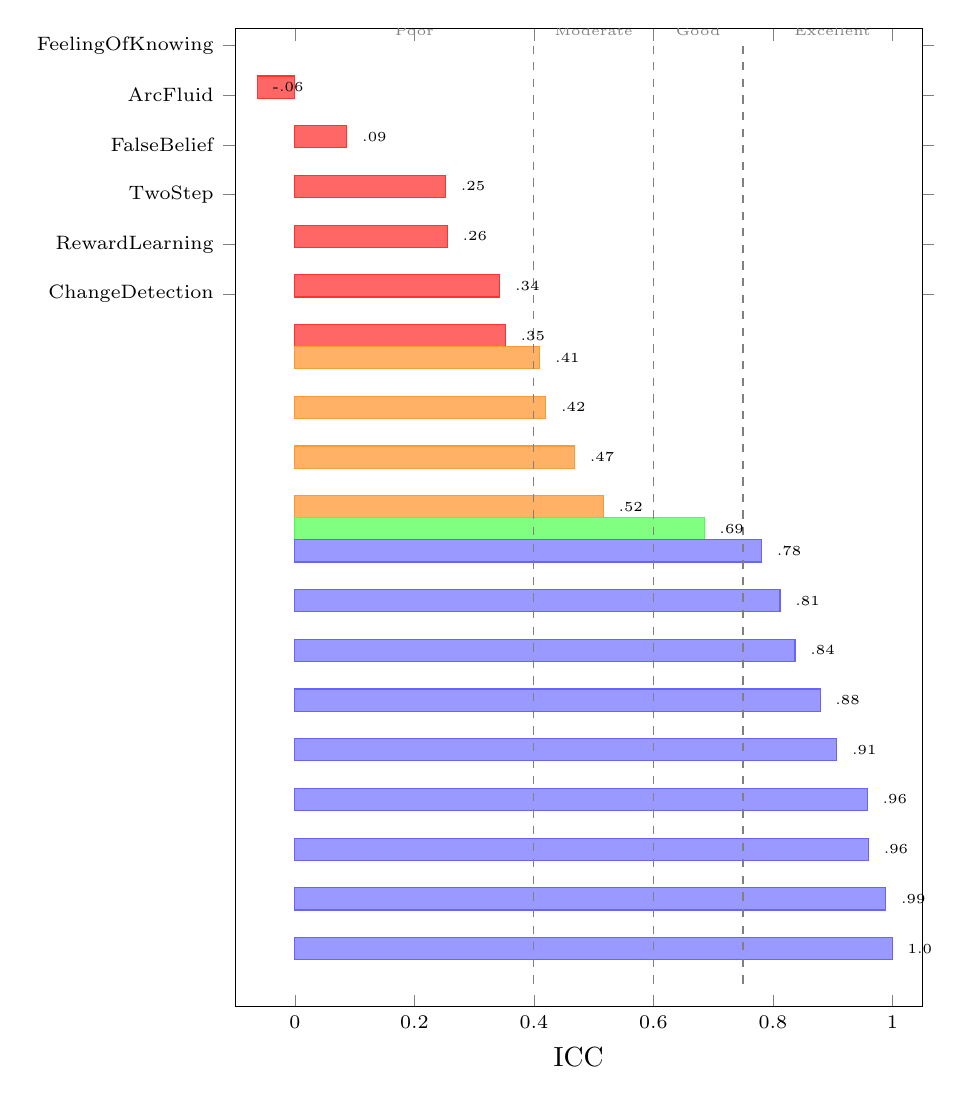
\begin{tikzpicture}
\begin{axis}[
    xbar,
    width=0.85\textwidth,
    height=14cm,
    xlabel={ICC},
    xmin=-0.1, xmax=1.05,
    ytick=data,
    y dir=reverse,
    symbolic y coords={
      FeelingOfKnowing,
      ArcFluid,
      FalseBelief,
      TwoStep,
      RewardLearning,
      ChangeDetection,
      SRTT,
      LexicalDecision,
      IGT,
      YerkesDodson,
      VisualSearch,
      Flanker,
      StopSignal,
      N-back,
      BART,
      WCST,
      Stroop,
      Calibration,
      ReversalLearning,
      DigitSpan},
    y tick label style={font=\scriptsize},
    x tick label style={font=\scriptsize},
    bar width=8pt,
    nodes near coords,
    nodes near coords style={font=\tiny, anchor=west},
    every node near coord/.append style={xshift=2pt},
    point meta=explicit symbolic,
    enlarge y limits={abs=6pt},
]
% Poor (ICC < 0.40)
\addplot[fill=red!60, draw=red!80] coordinates {
  (-0.063,FeelingOfKnowing) [-.06]
  (0.087,ArcFluid) [.09]
  (0.252,FalseBelief) [.25]
  (0.255,TwoStep) [.26]
  (0.343,RewardLearning) [.34]
  (0.352,ChangeDetection) [.35]
};
% Moderate (0.40-0.59)
\addplot[fill=orange!60, draw=orange!80] coordinates {
  (0.410,SRTT) [.41]
  (0.420,LexicalDecision) [.42]
  (0.468,IGT) [.47]
  (0.516,YerkesDodson) [.52]
};
% Good (0.60-0.74)
\addplot[fill=green!50, draw=green!70] coordinates {
  (0.685,VisualSearch) [.69]
};
% Excellent (>= 0.75) -- split for color
\addplot[fill=blue!40, draw=blue!60] coordinates {
  (0.781,Flanker) [.78]
  (0.812,StopSignal) [.81]
  (0.837,N-back) [.84]
  (0.879,BART) [.88]
  (0.907,WCST) [.91]
  (0.958,Stroop) [.96]
  (0.960,Calibration) [.96]
  (0.989,ReversalLearning) [.99]
  (1.000,DigitSpan) [1.0]
};
% Threshold lines
\draw[dashed, gray, thin] (axis cs:0.40,FeelingOfKnowing) -- (axis cs:0.40,DigitSpan);
\draw[dashed, gray, thin] (axis cs:0.60,FeelingOfKnowing) -- (axis cs:0.60,DigitSpan);
\draw[dashed, gray, thin] (axis cs:0.75,FeelingOfKnowing) -- (axis cs:0.75,DigitSpan);
\node[font=\tiny, gray, anchor=south] at (axis cs:0.20,FeelingOfKnowing) {Poor};
\node[font=\tiny, gray, anchor=south] at (axis cs:0.50,FeelingOfKnowing) {Moderate};
\node[font=\tiny, gray, anchor=south] at (axis cs:0.675,FeelingOfKnowing) {Good};
\node[font=\tiny, gray, anchor=south] at (axis cs:0.90,FeelingOfKnowing) {Excellent};
\end{axis}
\end{tikzpicture}
\caption{Test-retest reliability (ICC) for 20 evaluated benchmarks. Colors: red = Poor ($< 0.40$, $n = 6$), orange = Moderate ($0.40$--$0.59$, $n = 4$), green = Good ($0.60$--$0.74$, $n = 1$), blue = Excellent ($\geq 0.75$, $n = 9$). Dashed lines indicate class boundaries. Data from \texttt{reliability.csv}.}
\label{fig:icc}
\end{figure}

\clearpage
\section*{S4. Neuromodulator Dissociation Details and API Usage}

\subsection*{S4.1 Behavioral Knockout Effect Sizes}

The \texttt{BehavioralKnockout} benchmark reveals large, selective effects for each transmitter system:

\begin{itemize}
  \item \textbf{DA knockout}: reduces learning rate (Cohen's $d = 1.93$) and gradient tracking ($d = 2.14$)
  \item \textbf{NE knockout}: increases exploration ($d = 7.25$)
  \item \textbf{5-HT knockout}: reduces confidence ($d = 5.80$)
  \item \textbf{ACh knockout}: impairs attention ($d = 5.41$)
\end{itemize}

\noindent The \texttt{DoseResponse} benchmark shows perfect monotonicity (score $= 1.0$) for all five transmitter systems (DA, NE, 5-HT, ACh, GABA). \texttt{ToleranceWithdrawal} detects tolerance and withdrawal for all four tested transmitters (DA sensitivity ratio $= 0.48$, NE $= 0.59$, 5-HT $= 0.64$, GABA $= 0.73$). The theoretical prediction of four double dissociations---DA enhancing flexibility while impairing sustained attention, NE enhancing alerting while impairing fine motor control, 5-HT enhancing inhibition while slowing working memory, ACh enhancing focused attention while impairing flexibility---remains to be tested with a full profile $\times$ benchmark cross-tabulation in future work.

\subsection*{S4.2 API Usage}

\psychbench{} is distributed as a Rust crate (\texttt{symthaea-psych-bench}) and can be integrated into any project via Cargo. The API provides four levels of usage.

\paragraph{Single benchmark evaluation.} Running an individual benchmark requires constructing a configuration and calling \texttt{run()}:

\begin{verbatim}
use symthaea_psych_bench::benchmarks::executive::StroopBenchmark;
use symthaea_psych_bench::harness::{BenchmarkConfig, PsychBenchmark};

let config = BenchmarkConfig::default(); // seed=42, dim=512
let result = StroopBenchmark.run(&config);
println!("Stroop effect: {:.3}", result.metrics["stroop_effect"].mean);
\end{verbatim}

\paragraph{Full battery with cognitive profile.} The harness aggregates results into an 8-domain cognitive profile:

\begin{verbatim}
use symthaea_psych_bench::harness::{BenchmarkReport, CognitiveProfile};

let mut report = BenchmarkReport::new();
for bench in &all_benchmarks {
    report.add(bench.run(&config));
}
let profile = CognitiveProfile::from_report(&report);
\end{verbatim}

\paragraph{HTML report generation.}

\begin{verbatim}
use symthaea_psych_bench::harness::html::HtmlReport;

let html = HtmlReport::from_report(&report);
std::fs::write("report.html", html.render()).unwrap();
\end{verbatim}

\paragraph{Neuromodulator sweep.} Pharmacological profiles can be applied to any benchmark subset:

\begin{verbatim}
use symthaea_psych_bench::harness::neuromod_profiles::NeuromodProfile;

for profile in NeuromodProfile::standard_profiles() {
    let mut config = BenchmarkConfig::default();
    config.label = Some(profile.name.clone());
    let result = StroopBenchmark.run(&config);
}
\end{verbatim}

\noindent All APIs are deterministic given a fixed seed, enabling exact replication. Full API documentation is generated via \texttt{cargo doc -p symthaea-psych-bench}.

% ============================================================
% Section S6: Neuromodulator Behavioral Dissociations
% ============================================================

\clearpage
\section*{S6. Neuromodulator Behavioral Dissociations}

Selective transmitter knockout in the \texttt{BehavioralKnockout} benchmark produces large, dissociable effects on distinct behavioral measures. Table~S3 summarizes the Cohen's $d$ effect sizes for each transmitter $\times$ behavioral measure combination. Each transmitter primarily disrupts one or two measures while leaving others largely unaffected, consistent with the functional specialization reported in the psychopharmacological literature \citep{schultz1997dopamine,yerkes1908relation}.

\begin{table}[h]
\centering
\caption{Behavioral knockout effect sizes (Cohen's $d$). Bold values indicate the primary (largest magnitude) effect for each transmitter. Empty cells denote non-primary effects ($d < 0.5$).} \label{tab:s3}
\begin{tabular}{@{}lccccc@{}}
\toprule
\textbf{Transmitter} & \textbf{Learning Rate} & \textbf{Exploration} & \textbf{Confidence} & \textbf{Attention} & \textbf{Gradient Tracking} \\
\midrule
DA  & 1.93 & --- & --- & --- & \textbf{2.14} \\
NE  & --- & \textbf{7.25} & --- & --- & --- \\
5-HT & --- & --- & \textbf{5.80} & --- & --- \\
ACh & --- & --- & --- & \textbf{5.41} & --- \\
\bottomrule
\end{tabular}
\end{table}

\noindent The large effect sizes ($d > 1.9$ for all primary effects) confirm that each neuromodulator system has a distinct functional role within the architecture: dopamine gates reward-driven learning and gradient tracking, norepinephrine modulates exploration--exploitation balance, serotonin regulates prediction confidence, and acetylcholine controls attentional gain. The simultaneous knockout of all four transmitters produces a consciousness collapse ($d = 9.43$), indicating that neuromodulatory tone is necessary for maintaining integrated conscious processing.

\subsection*{S6.1 Dose--Response and Tolerance Dynamics}

Table~S4 summarizes dose--response monotonicity and tolerance/withdrawal sensitivity ratios across the four primary transmitter systems plus GABA. All transmitters exhibit perfect monotonicity (score $= 1.0$), confirming that behavioral effects scale smoothly with concentration. The sensitivity ratio (post-tolerance response / initial response) indicates the degree of adaptation under sustained exposure: lower ratios reflect stronger tolerance development.

\begin{table}[h]
\centering
\caption{Dose--response monotonicity and tolerance/withdrawal sensitivity ratios. Data from \texttt{DoseResponse} and \texttt{ToleranceWithdrawal} benchmarks.} \label{tab:s4}
\begin{tabular}{@{}lcc@{}}
\toprule
\textbf{Transmitter} & \textbf{Monotonicity} & \textbf{Sensitivity Ratio} \\
\midrule
DA   & 1.0 & 0.48 \\
NE   & 1.0 & 0.59 \\
5-HT & 1.0 & 0.64 \\
GABA & 1.0 & 0.73 \\
\bottomrule
\end{tabular}
\end{table}

\noindent Dopamine shows the strongest tolerance (ratio $= 0.48$), consistent with clinical observations of dopaminergic adaptation in reward circuits. GABA shows the weakest tolerance (ratio $= 0.73$), reflecting its role as a tonic inhibitory baseline. All four transmitters show detectable withdrawal effects upon cessation.

\clearpage
\section*{S5. Per-Domain Ablation Analysis}

Table~S5 shows per-domain z-scores under six ablation presets. FullConsciousness is the baseline (all subsystems active). Each preset disables or degrades one subsystem, operationalized as increased encoding noise. Domains with identical scores across all presets (e.g., InstitutionalReasoning, Security) rely on structural HDC operations unaffected by encoding noise.

\renewcommand{\arraystretch}{1.15}
\begin{longtable}{@{}lrrrrrrr@{}}
\caption{Per-domain z-scores under six ablation presets. \textbf{Bold} indicates $|\Delta| > 0.5$ from the FullConsciousness baseline. Max~$\Delta$ is the range (max $-$ min) across all six presets.} \label{tab:s5} \\
\toprule
\textbf{Domain} & \textbf{Full} & \textbf{CfCOnly} & \textbf{NoFEP} & \textbf{NoSocial} & \textbf{RedWM} & \textbf{HDCOnly} & \textbf{Max~$\Delta$} \\
\midrule
\endfirsthead
\toprule
\textbf{Domain} & \textbf{Full} & \textbf{CfCOnly} & \textbf{NoFEP} & \textbf{NoSocial} & \textbf{RedWM} & \textbf{HDCOnly} & \textbf{Max~$\Delta$} \\
\midrule
\endhead
\midrule
\multicolumn{8}{r}{\emph{Continued on next page}} \\
\endfoot
\bottomrule
\endlastfoot
Affect & 1.20 & 1.22 & 1.22 & 1.22 & 0.77 & 0.76 & 0.46 \\
Attention & 0.68 & 0.44 & 0.52 & 0.62 & 0.29 & \textbf{0.04} & 0.64 \\
Binding & 0.62 & 0.62 & 0.61 & 0.61 & 0.62 & 0.62 & 0.01 \\
Butlin & 0.67 & 0.67 & 0.67 & 0.67 & 0.67 & 0.67 & 0.00 \\
CausalReasoning & 0.80 & 0.80 & 0.80 & 0.80 & 0.80 & 0.80 & 0.00 \\
Clinical & 2.00 & 1.83 & 1.91 & 1.91 & 1.89 & 1.77 & 0.23 \\
Coding & 1.86 & 1.98 & 1.95 & 1.90 & 1.97 & 2.00 & 0.15 \\
CogBench & 0.58 & 0.58 & 0.58 & 0.58 & 0.58 & 0.58 & 0.00 \\
Consciousness & 0.69 & 0.66 & 0.66 & 0.69 & 0.65 & 0.61 & 0.08 \\
Creativity & 0.67 & 0.84 & 0.84 & 0.76 & 0.79 & 0.87 & 0.19 \\
Executive & 0.72 & 0.36 & 0.49 & 0.68 & 0.50 & \textbf{0.13} & 0.59 \\
Inhibition & 1.57 & \textbf{0.22} & \textbf{0.81} & 1.20 & \textbf{0.58} & \textbf{$-$0.53} & 2.10 \\
InstitutionalReasoning & 2.25 & 2.25 & 2.25 & 2.25 & 2.25 & 2.25 & 0.00 \\
Language & 1.75 & \textbf{0.26} & \textbf{1.24} & 1.75 & 1.73 & \textbf{$-$0.76} & 2.51 \\
Mathematics & 1.25 & \textbf{0.49} & \textbf{0.47} & 0.92 & \textbf{0.45} & \textbf{$-$0.36} & 1.61 \\
MemoryAgent & 1.00 & 1.00 & 1.00 & 1.00 & \textbf{0.22} & \textbf{0.22} & 0.78 \\
Metacognition & 0.75 & 0.55 & 0.60 & 0.68 & 0.66 & 0.67 & 0.21 \\
Motor & 2.32 & 2.15 & 2.20 & 2.25 & 2.18 & 2.07 & 0.25 \\
Reasoning & 1.39 & 1.38 & 1.38 & 1.39 & 1.38 & 1.37 & 0.02 \\
Security & 2.00 & 2.00 & 2.00 & 2.00 & 2.00 & 2.00 & 0.00 \\
Social & 1.54 & \textbf{0.67} & 1.43 & \textbf{0.95} & 1.40 & \textbf{0.42} & 1.12 \\
Spatial & 1.21 & 1.21 & 1.21 & 1.21 & 1.21 & 1.21 & 0.00 \\
Speech & 2.13 & 1.96 & 2.14 & 2.13 & 2.20 & \textbf{0.30} & 1.90 \\
Substrate & 0.88 & 0.96 & 0.94 & 0.92 & 0.95 & 0.99 & 0.11 \\
SustainedAttention & 2.19 & 2.19 & 2.19 & 2.19 & 2.19 & 2.19 & 0.00 \\
ToMBench & 1.08 & 1.08 & 1.08 & 1.08 & 1.08 & 1.08 & 0.00 \\
WorM & 0.73 & 0.56 & 0.67 & 0.67 & \textbf{$-$2.36} & \textbf{$-$2.36} & 3.09 \\
\end{longtable}

\bibliographystyle{apalike}
\bibliography{psych_bench_references}

\end{document}
